%************************************************
\section{The Design} % (fold)
\label{sec:the_design}
%************************************************
To summarize, we present an overview of our design. We will represent the target environment as a 3D virtual model \ref{sec:simulation_designer}. We will build a simulation runtime based on a game engine \ref{sec:simulation_runtime}. To empower the simulation user to interact with the environment, we will build an agent based on a first-person perspective. The agent will be controlled using standard game controls as described in Section \ref{sec:the_agent}. As the agent is interacting with the environment the monitoring service \ref{sec:monitoring_service} will classify objects around the agent according to the Situative Space Model (SSM). The content of the SSM sets will be available for third party services through a RESTful API \ref{sec:api} and for the simulation user, in a visual representation, through the context client \ref{sec:context_client}. Figure \ref{fig:final_architecture} show a visual overview of this design. It is a more concrete design than the one presented in the begging of this chapter \ref{fig:initial_architecture}. We have modified the initial design to fit the architecture of a game engine illustrated in Figure \ref{fig:game_engine_architecture}.
\begin{figure}[H]
	\centering
	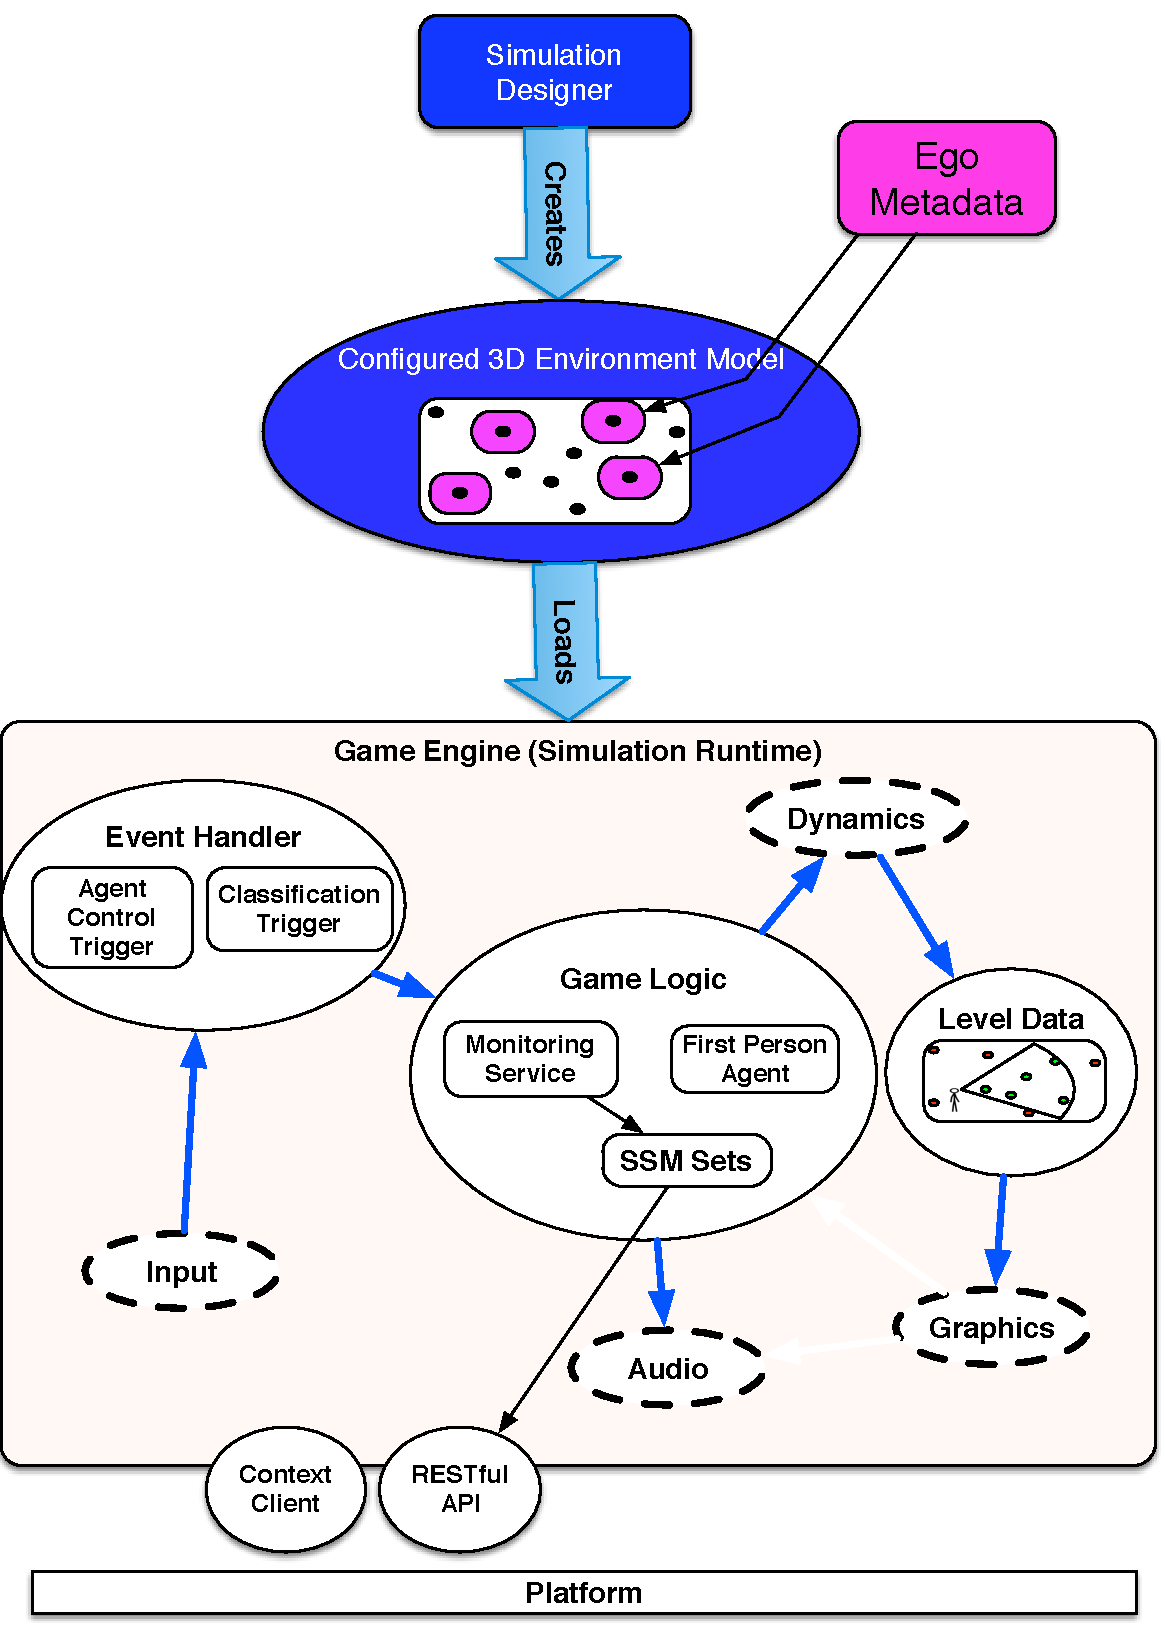
\includegraphics[width=\linewidth]{gfx/Chapter3/final_architecture}
	\caption{EgoSim: A visual overview of our final architecture}
	\label{fig:final_architecture}
\end{figure}
% section the_design (end)